\newcommand{\NWtarget}[2]{#2}
\newcommand{\NWlink}[2]{#2}
\newcommand{\NWtxtMacroDefBy}{Fragment defined by}
\newcommand{\NWtxtMacroRefIn}{Fragment referenced in}
\newcommand{\NWtxtMacroNoRef}{Fragment never referenced}
\newcommand{\NWtxtDefBy}{Defined by}
\newcommand{\NWtxtRefIn}{Referenced in}
\newcommand{\NWtxtNoRef}{Not referenced}
\newcommand{\NWtxtFileDefBy}{File defined by}
\newcommand{\NWtxtIdentsUsed}{Uses:}
\newcommand{\NWtxtIdentsNotUsed}{Never used}
\newcommand{\NWtxtIdentsDefed}{Defines:}
\newcommand{\NWsep}{${\diamond}$}
\newcommand{\NWnotglobal}{(not defined globally)}
\newcommand{\NWuseHyperlinks}{}
\documentclass{article}
\usepackage{graphicx, color}
\usepackage{hyperref}
\usepackage{tikz}
\usepackage{pgf-umlcd}
\title{\color{blue}P5.19}
\author{\color{blue}Frank Mock}
\date{\color{blue}October 10, 2011}
\begin{document}
\maketitle
\section{Specification}
	Design a class Cannonball to model a cannonball that is fired into the air. 
    A ball has an x and a y position and an x and y velocity
		
	Supply the following member functions:
		\begin{itemize}
		\item	A constructor with a weight and an x-position (the y-position is initially 0)
		\item	A member function move(double sec) that moves the ball to the next position (First compute 
                the distance traveled in sec seconds, using the current velocities, then update the x- and y-positions; 
                then update the y-velocity by taking into account the gravitational acceleration of - 9.81 m/sec2; the 
                x-velocity is unchanged.)
		\item	A member function plot that plots the current location of the cannonball
		\item	A member function shoot whose parameters are the angle a and initial velocity v 
                (Compute the x-velocity as v cos a and the y-velocity as v sin a; then keep calling move with a time 
                interval of 0.1 seconds until the y-position is 0; call plot after every move.)
		\end{itemize}
		
	Use this class in a program that prompts the user for the starting angle and the initial velocity. Then call shoot.

\section{Design}
	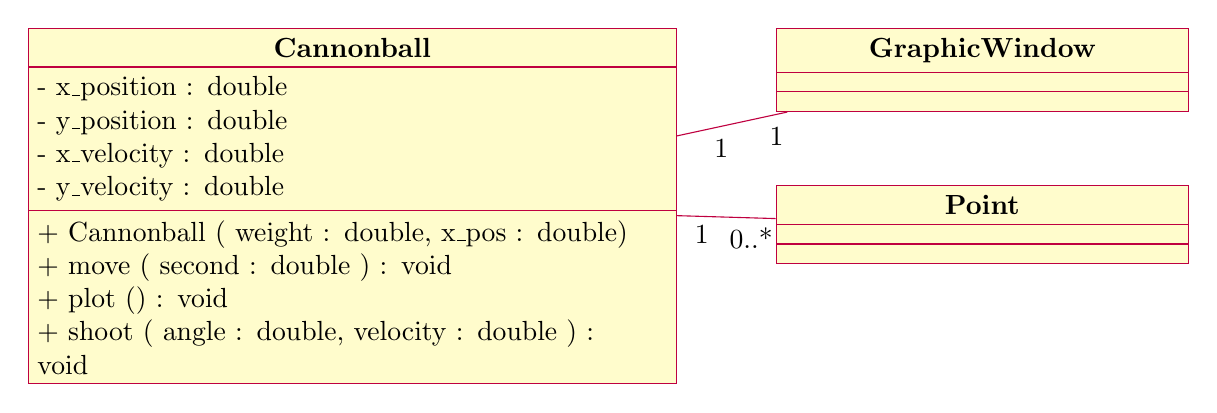
\begin{tikzpicture}
	\begin{class}[text width=8cm]{Cannonball}{0,0}
	\attribute {- x\_position : double}
	\attribute {- y\_position : double}
	\attribute {- x\_velocity : double}
	\attribute {- y\_velocity : double}
	\operation {+ Cannonball ( weight : double, x\_pos : double) }
	\operation {+ move ( second : double ) : void }
	\operation {+ plot () : void }
	\operation {+ shoot ( angle : double, velocity : double ) : void }
	\end{class}
	\begin{class}{GraphicWindow}{8,0}
	\end{class}
	\begin{class}{Point}{8,-2}
	\end{class}
	\association{Cannonball}{}{1} {GraphicWindow}{}{1}
	\association{Cannonball}{}{1} {Point}{}{0..*}
	\end{tikzpicture}
The velocity can be split into x and y components using these formulas from trigonometery

\begin{tikzpicture}
\draw(0,0)rectangle(4,8);
\draw(3.5,0)rectangle(4,0.5);
\draw(0.5,0.5)node[]{$\alpha$};
\draw(2,-0.5)node[]{$v \times \cos \alpha$};
\draw(5,4)node[]{$v \times \sin \alpha$};
\draw[->] (0,0) -- (4,8);
\end{tikzpicture}\\


\section{Implementation}
g is the gravitational acceleration of $-9.81 \frac{m}{sec*2}$.
a good approximation of $\pi$ is $ 4 \times \arctan 1.0$ Which we will
need to convert from the angle in degrees to the angle in radians.
The c++ sin and cos functions expect the argument to be in radians.
\begin{flushleft} \small
\begin{minipage}{\linewidth}\label{scrap1}\raggedright\small
\NWtarget{nuweb3}{} \verb@"cannonball.h"@\nobreak\ {\footnotesize {3}}$\equiv$
\vspace{-1ex}
\begin{list}{}{} \item
\mbox{}\verb@@\\
\mbox{}\verb@#include"ccc_win.h"@\\
\mbox{}\verb@#include<cmath>@\\
\mbox{}\verb@const double g = -9.81; //m/sec x sec@\\
\mbox{}\verb@const double pi = 4 * atan(1.0);@\\
\mbox{}\verb@class Cannonball@\\
\mbox{}\verb@{@\\
\mbox{}\verb@private:@\\
\mbox{}\verb@  double x_position;@\\
\mbox{}\verb@  double y_position;@\\
\mbox{}\verb@  double x_velocity;@\\
\mbox{}\verb@  double y_velocity;@\\
\mbox{}\verb@public:@\\
\mbox{}\verb@  Cannonball(double w, double x);@\\
\mbox{}\verb@  void move(double s);@\\
\mbox{}\verb@  void plot() const;@\\
\mbox{}\verb@  void shoot(double a, double v);@\\
\mbox{}\verb@};@\\
\mbox{}\verb@@{\NWsep}
\end{list}
\vspace{-1.5ex}
\footnotesize
\begin{list}{}{\setlength{\itemsep}{-\parsep}\setlength{\itemindent}{-\leftmargin}}

\item{}
\end{list}
\end{minipage}\vspace{4ex}
\end{flushleft}
Assume the initial y position is always zero (starting from the ground)
Weight does not seem to affect the trijectory, but we store it for possible later
use. Use the Point class from the authors graphic library to indicate the positions
that the cannonball is in as it moves through its trajectory.
\begin{flushleft} \small
\begin{minipage}{\linewidth}\label{scrap2}\raggedright\small
\NWtarget{nuweb4a}{} \verb@"cannonball.cpp"@\nobreak\ {\footnotesize {4a}}$\equiv$
\vspace{-1ex}
\begin{list}{}{} \item
\mbox{}\verb@@\\
\mbox{}\verb@#include"cannonball.h"@\\
\mbox{}\verb@Cannonball::Cannonball(double w, double x)@\\
\mbox{}\verb@{@\\
\mbox{}\verb@ x_position = x;@\\
\mbox{}\verb@ y_position = 0;@\\
\mbox{}\verb@ x_velocity = 0;@\\
\mbox{}\verb@ y_velocity = 0;@\\
\mbox{}\verb@}@\\
\mbox{}\verb@void Cannonball::move(double s)@\\
\mbox{}\verb@{@\\
\mbox{}\verb@  x_position++;@\\
\mbox{}\verb@}@\\
\mbox{}\verb@/**@\\
\mbox{}\verb@Use the Point class from the authors graphic library @\\
\mbox{}\verb@to indicate the positions that the cannonball@\\
\mbox{}\verb@is in as it moves through its trajectory.@\\
\mbox{}\verb@*/@\\
\mbox{}\verb@void Cannonball::plot() const@\\
\mbox{}\verb@{@\\
\mbox{}\verb@ @\\
\mbox{}\verb@}@\\
\mbox{}\verb@void Cannonball::shoot(double a, double v)@\\
\mbox{}\verb@{@\\
\mbox{}\verb@  do@\\
\mbox{}\verb@  {@\\
\mbox{}\verb@    move(0.1);@\\
\mbox{}\verb@  }while(x_position < 50);@\\
\mbox{}\verb@}@\\
\mbox{}\verb@@{\NWsep}
\end{list}
\vspace{-1.5ex}
\footnotesize
\begin{list}{}{\setlength{\itemsep}{-\parsep}\setlength{\itemindent}{-\leftmargin}}

\item{}
\end{list}
\end{minipage}\vspace{4ex}
\end{flushleft}
In the main program, we create a cannonball, get initial angle and velocity from user
then call shoot
\begin{flushleft} \small
\begin{minipage}{\linewidth}\label{scrap3}\raggedright\small
\NWtarget{nuweb4b}{} \verb@"p5_19.cpp"@\nobreak\ {\footnotesize {4b}}$\equiv$
\vspace{-1ex}
\begin{list}{}{} \item
\mbox{}\verb@@\\
\mbox{}\verb@#include"cannonball.h"@\\
\mbox{}\verb@@\hbox{$\langle\,${\it Include Files}\nobreak\ {\footnotesize \NWlink{nuweb5a}{5a}}$\,\rangle$}\verb@@\\
\mbox{}\verb@int ccc_win_main()@\\
\mbox{}\verb@{@\\
\mbox{}\verb@ Cannonball c(10, 20);@\\
\mbox{}\verb@ double angle = cwin.get_double("Enter the launch angle in degrees: ");@\\
\mbox{}\verb@ double velocity = cwin.get_double("Enter the initial velocity in m/s:");@\\
\mbox{}\verb@ c.shoot(angle,velocity);@\\
\mbox{}\verb@ cwin << Message(Point(0,0),"Test");@\\
\mbox{}\verb@return 0;@\\
\mbox{}\verb@}@\\
\mbox{}\verb@@{\NWsep}
\end{list}
\vspace{-1.5ex}
\footnotesize
\begin{list}{}{\setlength{\itemsep}{-\parsep}\setlength{\itemindent}{-\leftmargin}}

\item{}
\end{list}
\end{minipage}\vspace{4ex}
\end{flushleft}
\begin{flushleft} \small
\begin{minipage}{\linewidth}\label{scrap4}\raggedright\small
\NWtarget{nuweb5a}{} $\langle\,${\it Include Files}\nobreak\ {\footnotesize {5a}}$\,\rangle\equiv$
\vspace{-1ex}
\begin{list}{}{} \item
\mbox{}\verb@@\\
\mbox{}\verb@#include "ccc_win.h"@\\
\mbox{}\verb@@{\NWsep}
\end{list}
\vspace{-1.5ex}
\footnotesize
\begin{list}{}{\setlength{\itemsep}{-\parsep}\setlength{\itemindent}{-\leftmargin}}
\item \NWtxtMacroRefIn\ \NWlink{nuweb4b}{4b}.

\item{}
\end{list}
\end{minipage}\vspace{4ex}
\end{flushleft}
\begin{flushleft} \small
\begin{minipage}{\linewidth}\label{scrap5}\raggedright\small
\NWtarget{nuweb5b}{} \verb@"p5_19.bat"@\nobreak\ {\footnotesize {5b}}$\equiv$
\vspace{-1ex}
\begin{list}{}{} \item
\mbox{}\verb@@\\
\mbox{}\verb@g++ -mwindows -I C:\C++_Programs\CS-116\cannonball\cccfiles -o p5_19 p5_19.cpp cannonball.cpp ^@\\
\mbox{}\verb@C:\C++_Programs\CS-116\cannonball\cccfiles\ccc_msw.cpp ^@\\
\mbox{}\verb@C:\C++_Programs\CS-116\cannonball\cccfiles\ccc_shap.cpp ^@\\
\mbox{}\verb@-lgdi32@\\
\mbox{}\verb@@{\NWsep}
\end{list}
\vspace{-1.5ex}
\footnotesize
\begin{list}{}{\setlength{\itemsep}{-\parsep}\setlength{\itemindent}{-\leftmargin}}

\item{}
\end{list}
\end{minipage}\vspace{4ex}
\end{flushleft}
\end{document}
